\chapter{\hlc[red]{Vida Decision Support System}} \label{ch:vida}



\section{\hlc[yellow]{Study Area \& Context}}

As the coronavirus pandemic swept the globe, many of the local points of contact working with Space Enabled on \ac{evdt} and other projects had sudden changes in priorities. Several of them raised the possibility of adapting and expanding the \ac{evdt} Modeling Framework to approach coronavirus-related decision-making and impact analysis. This seemed relevant because, as others have noted, coronavirus impacts and response can be characterized as a complex system warranting a multi-domain, model-based approach \cite{deweckHandlingCOVID192020}. The second case study will focus on this project, which ultimately became known as Vida and came to involve six metropolitan areas across Angola, Brazil, Chile, Indonesia, Mexico, and the United States. In each of these areas, Vida was (and is) developed in collaboration with local government officials, university researchers, and general community members. 

Whereas the first case study focuses on simulating the changes in mangrove forest over decades, the focus of Vida is examining hourly to weekly air and water quality data alongside daily coronavirus epidemiological data and weekly quarantine policies. Government officials need actionable data to both address the ongoing public health crisis and to cope with the resultant socioeconomic and environmental consequences. Community members need to understand why their government is making the decisions that it is and understand the risks associated with their own actions. \color{OliveGreen} The Technical Area Experts on this project include researchers from Harvard Medical School. Meanwhile the Local Area Experts (many of whom are technical experts in their own right) include a mix of government officials and academic researchers, most of whome work in the public health and/or in \ac{gis}. The intended Users are those same individuals as well as the various public health agencies / task forces that they are affiliated with.  In general, \color{black} the concept is for our partner organizations to use \ac{evdt} to develop analyses and presentations that can inform pandemic response. The exact process by which this takes place varies from location to location.

\subsection{\hlc[red]{Stakeholders}}

\section{\hlc[red]{Systems Architecture Framework}}

\subsection{\hlc[red]{Interviews}}

\subsection{\hlc[red]{Needs, Outcomes, and Objectives}}

\subsection{\hlc[red]{System Architecture}}

\begin{figure}[h]
	\centering
	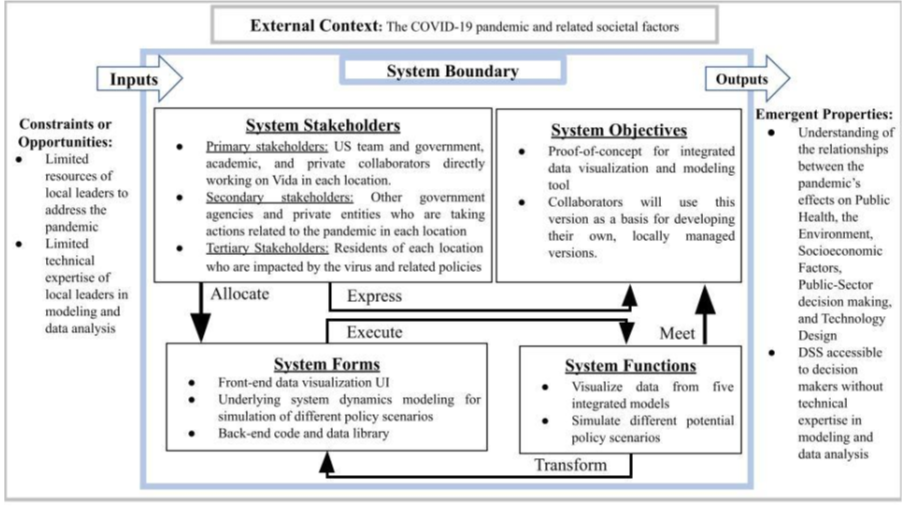
\includegraphics[scale=0.3]{/home/jackreid/Documents/School/Research/Space_Enabled/Thesis/Figures/architecture.png
}
	\caption{The high-level functional systems architecture of the Vida \ac{dss}.}
	\label{fig:architecture}
\end{figure}


\section{\hlc[red]{Vida Variant of EVDT}}


\subsection{\hlc[red]{Environment:}}

\subsection{\hlc[red]{Public Health:}}


\subsection{\hlc[red]{Vulnerability}}

\subsection{\hlc[red]{Decision-making}}

\subsection{\hlc[red]{Technology}}

\section{\hlc[red]{Decision Support System}}

\section{\hlc[red]{Evaluation}}

\section{\hlc[red]{Discussion}}

